\chapter{Metalen: reacties met zuren en corrosie}\label{ch:g9:metals-acids-corrosion}

In een haven zit de stalen romp van een oude vissersboot vol oranje
roestvegen. Op de kade staat een verzinkt hek al dertig jaar in de regen
en glanst nog steeds dofgrijs. In een museum ligt een gouden ring die
drieduizend jaar begraven lag en nog even blinkt als op de dag dat hij
gemaakt werd. Niet alle metalen reageren op dezelfde manier op hun
omgeving: sommige worden aangetast door water, \omterm{def:g4:air-a-mixture-of-gases:air}{lucht} en zuren, andere
nauwelijks.

\begin{recall}
\omterm{def:g9:ions:ion}{Ionen} zijn geladen \omterm{def:g7:atoms-and-molecules:atom}{atomen}; metalen vormen \omterm{def:g9:ions:ion}{kationen} zoals \ce{Fe^{2+}},
\ce{Zn^{2+}}, \ce{Al^{3+}}, die je met \omterm{def:g9:ions:precipitate}{neerslagreacties} aantoont
(\cref{ch:g9:ions}). Een \omterm{def:g9:acids-bases-ph:acidic}{zure oplossing} bevat veel \ce{H+(aq)}-ionen
(\cref{ch:g9:acids-bases-ph}). Waterstof verbrandt met een blaffend
plofje bij de opening van een reageerbuis
(\cref{ch:g7:identifying-substances}).
\end{recall}

\begin{omfigure}
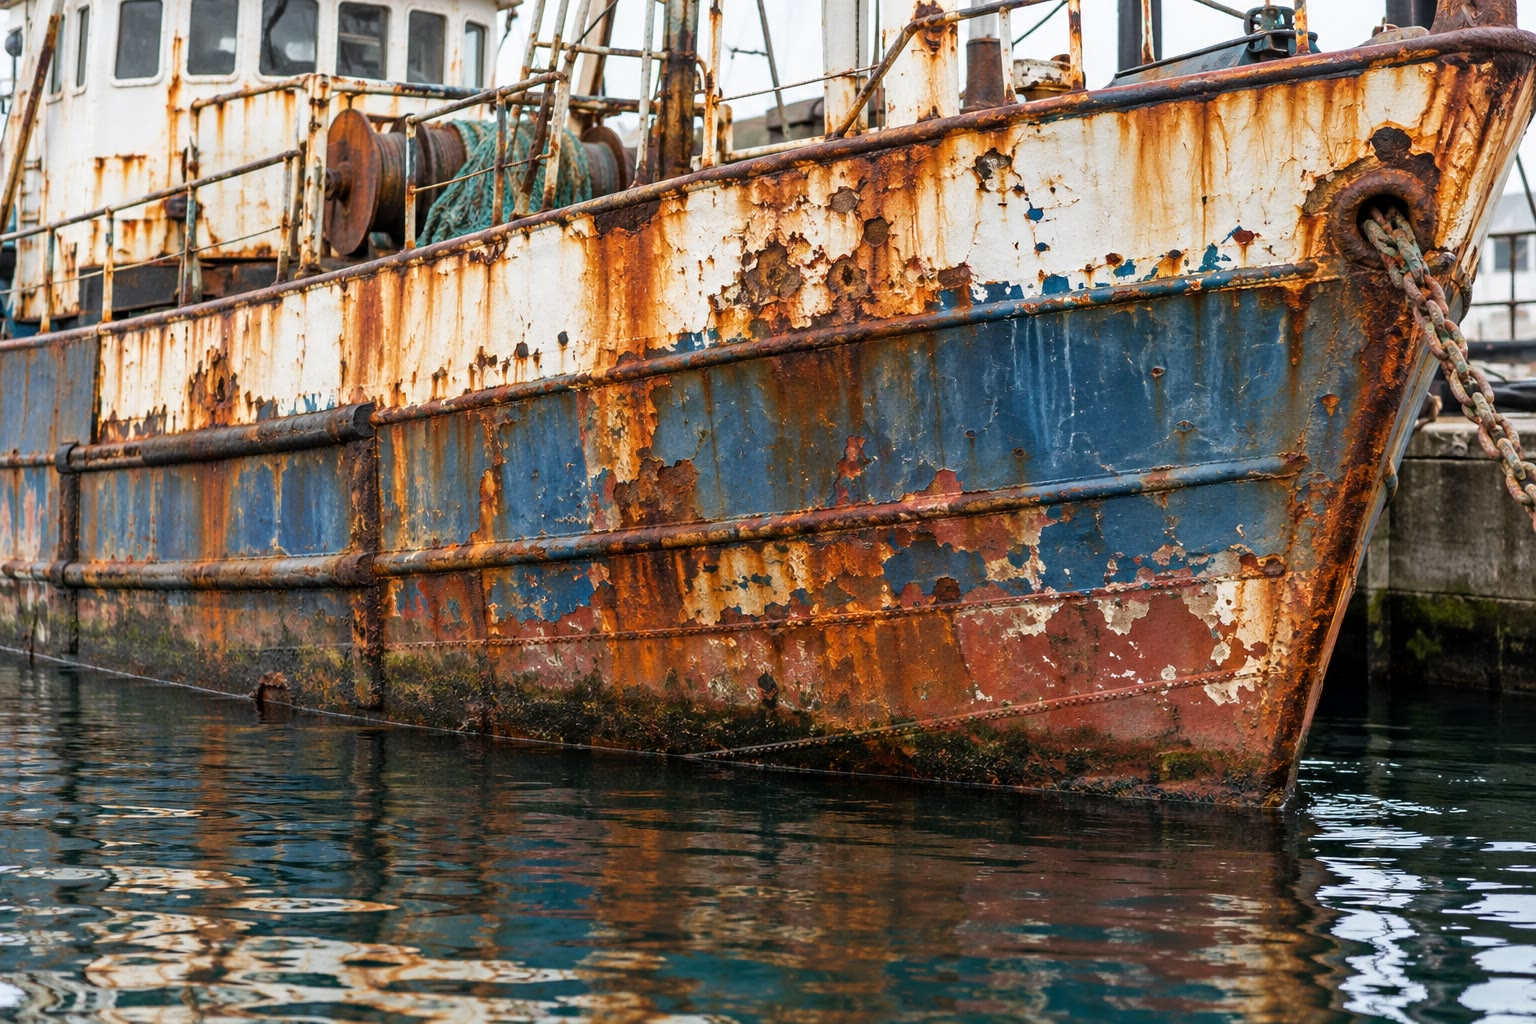
\includegraphics[width=0.55\linewidth]{images/book1/ai/g9-rusty-hull.jpg}

{\small De romp van een oude boot: het staal \omterm{def:g9:metals-acids-corrosion:corrosion}{roest}.}
\end{omfigure}

\section{Metalen in zoutzuur}

\begin{inthelab}[Drie metalen in zuur]
De docent laat een stukje ijzer, zink en koper vallen in drie
reageerbuizen met verdund zoutzuur. Bij het ijzer en het zink stijgen
belletjes op, langzaam bij het ijzer, flink bij het zink, en de metalen
verdwijnen langzaam; met het koper gebeurt niets. Het gas, opgevangen in
een buisje, geeft een blaffend plofje: het is waterstof. Met
natriumhydroxide geeft de vloeistof uit de eerste buis een groene
\omterm{def:g9:ions:precipitate}{neerslag} (\ce{Fe^{2+}}-ionen), die uit de tweede een witte
(\ce{Zn^{2+}}-ionen).
\end{inthelab}

\begin{omfigure}
\begin{tikzpicture}[font=\small, scale=1.2]
  \foreach \k/\m/\c/\bub in {0/ijzer/black!45/4, 1/zink/black!25/9, 2/koper/orange!60!brown/0} {
    \pic[transform shape] at (\k*2.4,0) {testtube={0.55}{omWater!70}};
    \fill[\c] (\k*2.4-0.13,0.08) rectangle (\k*2.4+0.13,0.35);
    \ifnum\bub>0
      \foreach \j in {1,...,\bub} {
        \pgfmathsetmacro\yy{0.45+0.12*\j}
        \pgfmathsetmacro\xx{\k*2.4+0.1*sin(97*\j)}
        \draw[black!55] (\xx,\yy) circle (0.035);
      }
    \fi
    \node[anchor=north, align=center] at (\k*2.4,-0.15) {\m};
  }
  \node[anchor=north, align=center, font=\footnotesize] at (0,-0.6) {belletjes, langzaam};
  \node[anchor=north, align=center, font=\footnotesize] at (2.4,-0.6) {belletjes, flink};
  \node[anchor=north, align=center, font=\footnotesize] at (4.8,-0.6) {geen reactie};
\end{tikzpicture}

{\small IJzer, zink en koper in verdund zoutzuur: ijzer en zink geven
waterstof af; koper reageert niet.}
\end{omfigure}

\begin{proposition}[Metaal plus zuur]\label{prop:g9:metals-acids-corrosion:acid}
Veel metalen --- ijzer, zink, aluminium, magnesium --- reageren met de
\ce{H+}-ionen van een zuur: het metaal verdwijnt als metaalionen, die
opgelost blijven, en er ontstaat waterstofgas. Koper, zilver en goud
reageren niet met zoutzuur.
\end{proposition}

\section{De reactievergelijking met ionen opschrijven}

\begin{definition}[Tribune-ion]\label{def:g9:metals-acids-corrosion:spectator}
Een \omterm{def:g9:ions:ion}{ion} dat tijdens een reactie in de oplossing aanwezig is maar er niet
aan meedoet, en aan het eind onveranderd terug te vinden is, is een
\emph{tribune-ion}\index{tribune-ion}. Je laat het weg uit de
\omterm{def:g8:balanced-equations:equation}{reactievergelijking}.
\end{definition}

\begin{example}[IJzer en zink in zoutzuur]\label{ex:g9:metals-acids-corrosion:iron}
Zoutzuur bevat \ce{H+(aq)}- en \ce{Cl-(aq)}-ionen. De \omterm{def:g9:ions:ion}{chloride-ionen} vind
je aan het eind onveranderd terug: het zijn \omterm{def:g9:metals-acids-corrosion:spectator}{tribune-ionen}. De
\omterm{def:g8:balanced-equations:equation}{reactievergelijkingen} zijn
\[
  \ce{Fe(s) + 2H+(aq) -> Fe^{2+}(aq) + H2(g)}, \qquad
  \ce{Zn(s) + 2H+(aq) -> Zn^{2+}(aq) + H2(g)}.
\]
Zowel de \omterm{def:g7:atoms-and-molecules:atom}{atomen} als de ladingen kloppen: aan elke kant $+2$.
\end{example}

\begin{method}[De reactievergelijking van een metaal met een zuur opschrijven]\label{met:g9:metals-acids-corrosion:write}
\begin{enumerate}
  \item \omterm{def:g7:chemical-reactions:reactant}{Beginstoffen}: het metaal (s) en de \ce{H+(aq)}-ionen.
  \item \omterm{def:g7:chemical-reactions:reactant}{Reactieproducten}: het metaalion (aq), met zijn gebruikelijke
        lading, en waterstof \ce{H2(g)}.
  \item Maak de \omterm{def:g7:atoms-and-molecules:atom}{atomen} kloppend, en controleer daarna of de totale lading
        aan beide kanten gelijk is.
\end{enumerate}
Voor aluminium: \ce{2Al(s) + 6H+(aq) -> 2Al^{3+}(aq) + 3H2(g)}; lading
$+6$ aan elke kant.
\end{method}

\begin{safety}{\ghs[0.8cm]{GHS02}\ghs[0.8cm]{GHS04}}
% ledger: ghs:H2
De waterstof die ontstaat, is zeer licht ontvlambaar. De reactie wordt
door de docent in kleine reageerbuizen uitgevoerd, ver van elke vlam
behalve die voor de knalgasproef.
\end{safety}

\section{Corrosie}

\begin{definition}[Corrosie en roest]\label{def:g9:metals-acids-corrosion:corrosion}
\emph{Corrosie}\index{corrosie} is de langzame aantasting van een metaal
door de stoffen om het heen --- zuurstof, water, zuren, zouten --- die het
metaal omzetten in \omterm{def:g9:ions:ion}{ionen} of in verbindingen zoals oxiden. Bij de
corrosie van ijzer en staal ontstaat \emph{roest}\index{roest}, een
bruin, kruimelig, gehydrateerd ijzeroxide dat afbladdert, zodat de
aantasting dieper kan doorgaan.
\end{definition}

\begin{proposition}[Wat ijzer nodig heeft om te roesten]\label{prop:g9:metals-acids-corrosion:needs}
IJzer \omterm{def:g9:metals-acids-corrosion:corrosion}{roest} alleen als zowel zuurstof als water erbij kan. Zout dat in
het water is opgelost, zoals op wegen die in de winter gestrooid worden
of aan zee, laat het \omterm{def:g9:metals-acids-corrosion:corrosion}{roesten} sneller gaan.
\end{proposition}

\begin{inthelab}[Drie spijkers, één week]
Drie schone ijzeren spijkers worden in drie reageerbuizen gezet: de
eerste met droge \omterm{def:g4:air-a-mixture-of-gases:air}{lucht} en een droogmiddel dat waterdamp wegneemt; de
tweede in water dat gekookt is om de opgeloste \omterm{def:g4:air-a-mixture-of-gases:air}{lucht} te verwijderen,
afgedekt met een laagje olie; de derde half in kraanwater, half in
\omterm{def:g4:air-a-mixture-of-gases:air}{lucht}. Na een week is alleen de derde spijker geroest.
\end{inthelab}

\begin{omfigure}
\begin{tikzpicture}[font=\small, scale=1.2]
  % tube 1: dry air, drying agent
  \pic[transform shape] at (0,0) {testtube={0.18}{white!80!black}};
  \foreach \x/\y in {-0.12/0.15,0.08/0.12,-0.02/0.3,0.12/0.32,-0.14/0.42,0.03/0.48}
    \fill[black!35] (\x,\y) circle (0.05);
  \fill[black!45] (-0.03,1.0) rectangle (0.03,2.4);
  \fill[black!45] (-0.09,2.4) rectangle (0.09,2.48);
  \fill[black!60] (-0.3,2.8) rectangle (0.3,3.1);
  \node[anchor=north, align=center] at (0,-0.15) {droge lucht:\\ geen roest};
  % tube 2: boiled water under oil
  \pic[transform shape] at (2.6,0) {testtube={0.7}{omWater!80}};
  \fill[yellow!55!orange!60] (2.36,1.85) rectangle (2.84,2.1);
  \fill[black!45] (2.57,0.3) rectangle (2.63,1.7);
  \fill[black!45] (2.51,1.7) rectangle (2.69,1.78);
  \fill[black!60] (2.3,2.8) rectangle (2.9,3.1);
  \node[anchor=north, align=center] at (2.6,-0.15) {water zonder lucht:\\ geen roest};
  % tube 3: water and air
  \pic[transform shape] at (5.2,0) {testtube={0.4}{omWater!80}};
  \fill[black!45] (5.17,0.3) rectangle (5.23,2.2);
  \fill[black!45] (5.11,2.2) rectangle (5.29,2.28);
  \fill[orange!60!brown] (5.15,0.9) rectangle (5.25,1.5);
  \node[anchor=north, align=center] at (5.2,-0.15) {water en lucht:\\ roest};
  \draw[<-, omProp, thick] (-0.15,0.3) -- (-0.9,0.7) node[left, text=black, font=\footnotesize] {droogmiddel};
  \draw[<-, omProp, thick] (2.85,1.98) -- (3.6,2.4) node[right, text=black, font=\footnotesize] {olie};
\end{tikzpicture}

{\small Het experiment met de drie spijkers: ijzer \omterm{def:g9:metals-acids-corrosion:corrosion}{roest} alleen waar
water en zuurstof er samen bij kunnen, hier aan het wateroppervlak.}
\end{omfigure}

\begin{example}[Aluminium en koper beschermen zichzelf]\label{ex:g9:metals-acids-corrosion:protect}
Aluminium wordt meteen aangetast door de zuurstof van de \omterm{def:g4:air-a-mixture-of-gases:air}{lucht}, maar het
dunne oxidelaagje dat ontstaat, hecht aan het metaal en sluit het af van
de \omterm{def:g4:air-a-mixture-of-gases:air}{lucht}: aluminium raamkozijnen gaan tientallen jaren mee. Koper, dat
langzaam wordt aangetast door \omterm{def:g4:air-a-mixture-of-gases:air}{lucht}, water en koolstofdioxide, raakt
bedekt met een groene korst, de patina, die ook hecht en het metaal
eronder beschermt. \omterm{def:g9:metals-acids-corrosion:corrosion}{Roest} daarentegen bladdert af.
\end{example}

\begin{omfigure}
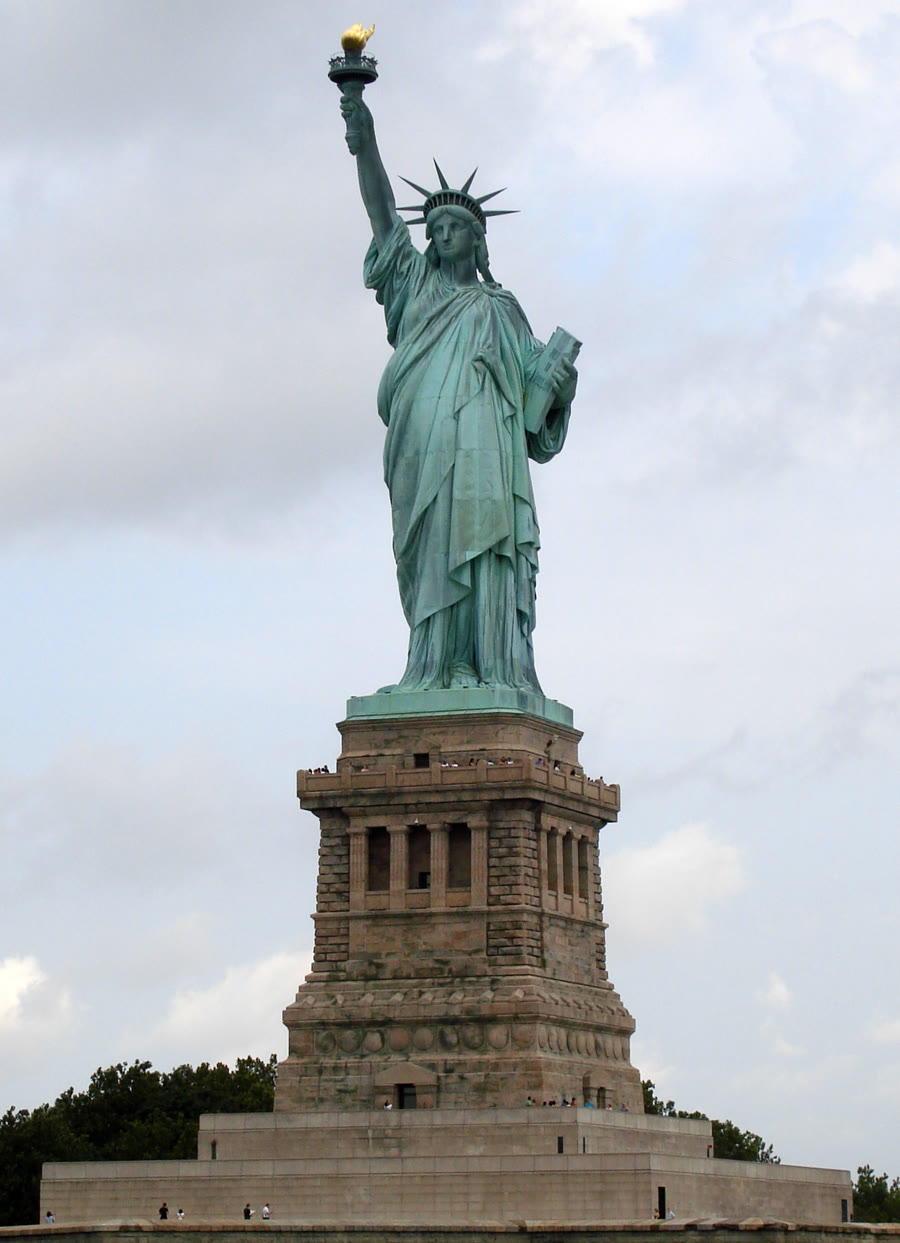
\includegraphics[height=6cm]{images/book1/statue-patina.jpg}

{\small Het Vrijheidsbeeld: zijn koperen huid is bedekt met een groene
patina. Foto: Elcobbola, publiek domein.}
\end{omfigure}

\section{Metalen beschermen}

\begin{definition}[Verzinken]\label{def:g9:metals-acids-corrosion:galvanising}
\emph{Verzinken}\index{verzinken} is staal bedekken met een laag zink,
door het in gesmolten zink te dompelen. \omterm{def:g4:air-a-mixture-of-gases:air}{Lucht} en water tasten dan het
zink aan in plaats van het staal eronder: zelfs waar de laag bekrast
is, corrodeert eerst het zink in de buurt en wordt het staal gespaard.
\end{definition}

\begin{proposition}[Manieren om ijzer en staal te beschermen]\label{prop:g9:metals-acids-corrosion:ways}
\begin{itemize}
  \item houd water en \omterm{def:g4:air-a-mixture-of-gases:air}{lucht} weg: verf, olie, vet, een kunststoflaag;
  \item verzink: een zinklaag die in plaats van het staal corrodeert;
  \item gebruik roestvast staal, een legering van ijzer met chroom, die
        zichzelf beschermt met een dun, afsluitend oxidelaagje;
  \item bevestig blokken zink aan scheepsrompen: het zink wordt langzaam
        weggevreten in plaats van het staal, en wordt af en toe vervangen
        (hoe dat werkt, legt een universiteitsdeel uit).
\end{itemize}
\end{proposition}

\begin{omfigure}
\begin{minipage}[b]{0.52\linewidth}\centering
\begin{tikzpicture}[font=\small]
  \fill[black!35] (0,0) rectangle (5,0.8);
  \fill[black!15] (0,0.8) rectangle (2.2,1.1);
  \fill[black!15] (2.8,0.8) rectangle (5,1.1);
  \fill[omWater!80] (1.6,1.1) rectangle (3.4,1.35);
  \fill[omWater!80] (2.2,0.8) rectangle (2.8,1.1);
  \draw[black!60] (0,0) rectangle (5,0.8);
  \foreach \x in {1.95,2.1} \draw[->, omProp, thick] (\x,1.25) -- (\x+0.05,1.7);
  \node[anchor=west, font=\footnotesize] at (5.1,0.4) {staal};
  \node[anchor=west, font=\footnotesize] at (5.1,0.95) {zinklaag};
  \node[anchor=south, font=\footnotesize, align=center] at (2.0,1.75) {zinkionen\\ gaan het water in};
  \node[anchor=north, font=\footnotesize, align=center] at (2.5,-0.05) {een kras: het staal\\ ligt bloot, maar het zink\\ eromheen corrodeert eerst};
\end{tikzpicture}

{\small Een bekraste verzinkte plaat.}
\end{minipage}\hfill
\begin{minipage}[b]{0.44\linewidth}\centering
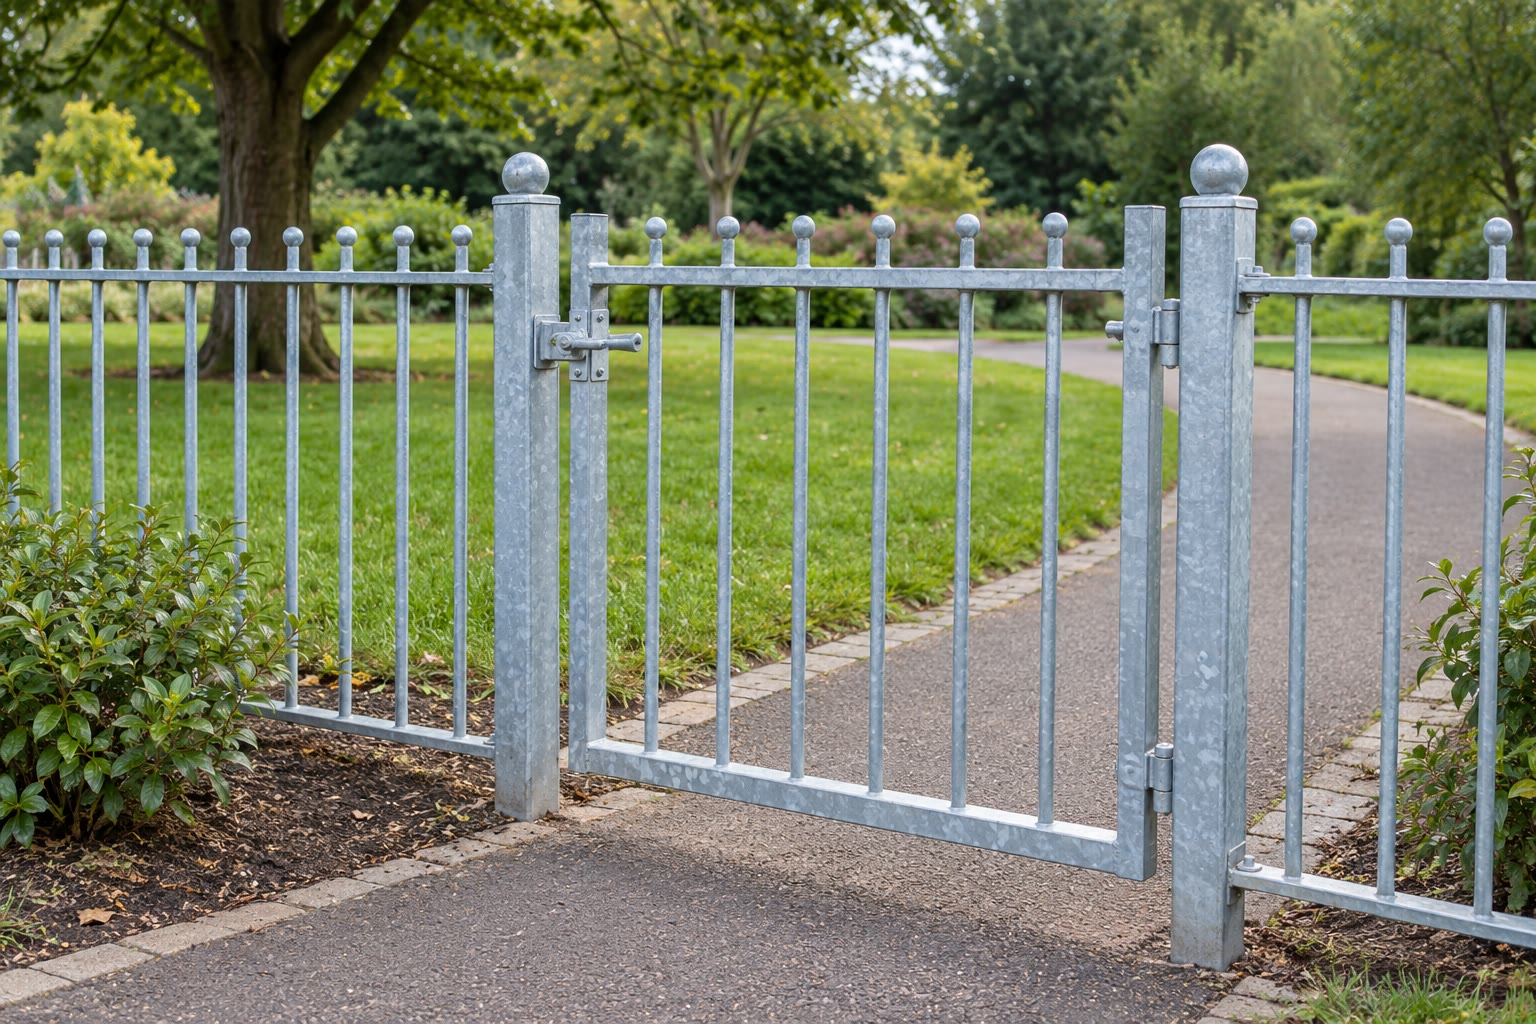
\includegraphics[width=\linewidth,height=4.4cm,keepaspectratio]{images/book1/ai/g9-galvanised-railings.jpg}

{\small Verzinkte stalen hekken.}
\end{minipage}
\end{omfigure}

\section{Oefeningen}

\begin{exercise}[$\star$]\label{exo:g9:metals-acids-corrosion:1}
Welk gas ontstaat er als zink met zoutzuur reageert? Hoe toon je het
aan?
\end{exercise}

\begin{exercise}[$\star$]\label{exo:g9:metals-acids-corrosion:2}
Welke van deze metalen reageren met verdund zoutzuur: ijzer, koper,
zink, goud, aluminium?
\end{exercise}

\begin{exercise}[$\star$]\label{exo:g9:metals-acids-corrosion:3}
Wat heeft ijzer nodig om te \omterm{def:g9:metals-acids-corrosion:corrosion}{roesten}?
\end{exercise}

\begin{exercise}[$\star$]\label{exo:g9:metals-acids-corrosion:4}
Wat is een \omterm{def:g9:metals-acids-corrosion:spectator}{tribune-ion}? Noem het \omterm{def:g9:metals-acids-corrosion:spectator}{tribune-ion} als ijzer met zoutzuur
reageert.
\end{exercise}

\begin{exercise}[$\star\star$]\label{exo:g9:metals-acids-corrosion:5}
Schrijf de \omterm{def:g8:balanced-equations:equation}{reactievergelijking} op van magnesium met de \ce{H+}-ionen van
een zuur (het magnesiumion is \ce{Mg^{2+}}). Controleer de ladingen.
\end{exercise}

\begin{exercise}[$\star\star$]\label{exo:g9:metals-acids-corrosion:6}
Hoe kun je, nadat ijzer met zoutzuur heeft gereageerd, laten zien dat
de oplossing ijzer(II)\omterm{def:g9:ions:ion}{ionen} bevat?
\end{exercise}

\begin{exercise}[$\star\star$]\label{exo:g9:metals-acids-corrosion:7}
Kijk naar de figuur met de drie spijkers. Waarom is het water in de
tweede buis gekookt en afgedekt met olie?
\end{exercise}

\begin{exercise}[$\star\star$]\label{exo:g9:metals-acids-corrosion:8}
Waarom \omterm{def:g9:metals-acids-corrosion:corrosion}{roest} een auto sneller in een stad waar de wegen in de winter
gestrooid worden?
\end{exercise}

\begin{exercise}[$\star\star$]\label{exo:g9:metals-acids-corrosion:9}
Waarom \omterm{def:g9:metals-acids-corrosion:corrosion}{roesten} aluminium raamkozijnen niet weg, hoewel aluminium met de
zuurstof van de \omterm{def:g4:air-a-mixture-of-gases:air}{lucht} reageert?
\end{exercise}

\begin{exercise}[$\star\star$]\label{exo:g9:metals-acids-corrosion:10}
Geef drie manieren om een stalen fietsframe tegen \omterm{def:g9:metals-acids-corrosion:corrosion}{roest} te beschermen.
\end{exercise}

\begin{exercise}[$\star\star\star$]\label{exo:g9:metals-acids-corrosion:11}
Schrijf de \omterm{def:g8:balanced-equations:equation}{reactievergelijking} op van aluminium met de \ce{H+}-ionen van
een zuur, en controleer haar. Hoeveel waterstofmoleculen ontstaan er
per 200 aluminiumatomen?
\end{exercise}

\begin{exercise}[$\star\star\star$]\label{exo:g9:metals-acids-corrosion:12}
In een verzinkte stalen emmer zit een kras tot op het staal. Leg uit
waarom het staal onder in de kras lange tijd niet \omterm{def:g9:metals-acids-corrosion:corrosion}{roest}.
\end{exercise}

\section{Probleem: Hoe dik is het zink?}

\begin{problem}[{Weekendprobleem --- de zinklaag van een verzinkte plaat
oplossen om te weten te komen hoe dik ze was}]
\label{pb:g9:metals-acids-corrosion:1}
% ledger: rho:Zn
Een verzinkte stalen plaat, een vierkant met zijde \qty{10.0}{cm}, is
aan beide kanten met zink bedekt (de randen worden verwaarloosd). In een
laboratorium weegt de docent haar, \qty{125.6}{g}, en dompelt haar dan in
zoutzuur waaraan een middel is toegevoegd dat voorkomt dat het zuur het
staal aantast. Als het bruisen ophoudt, wordt de plaat afgespoeld,
gedroogd en opnieuw gewogen: \qty{113.5}{g}. De massa van \qty{1}{cm^3}
zink is \qty{7.13}{g}.

\medskip
\noindent\textbf{Deel I --- De reactie.}
\begin{enumerate}
  \item Schrijf de \omterm{def:g8:balanced-equations:equation}{reactievergelijking} op van zink met de \ce{H+}-ionen
        van het zuur.
  \item Welk gas veroorzaakt het bruisen? Beschrijf de test ervoor.
  \item Met welke test zou je na afloop de zinkionen in de oplossing
        aantonen?
  \item Noem de \omterm{def:g9:metals-acids-corrosion:spectator}{tribune-ionen}.
\end{enumerate}

\medskip
\noindent\textbf{Deel II --- Het zink.}
\begin{enumerate}[resume]
  \item Hoeveel zink is er opgelost?
  \item Waarom is het bruisen een teken dat nog niet al het zink is
        opgelost?
  \item Wat zou er met het staal gebeuren als het zuur het middel niet
        bevatte? Welke test zou dat dan laten zien?
  \item Waarom beschermt het zink het staal van de plaat zolang het er
        is?
\end{enumerate}

\medskip
\noindent\textbf{Deel III --- De dikte.}
\begin{enumerate}[resume]
  \item Wat is de totale bedekte oppervlakte van de plaat, in
        \unit{cm^2}?
  \item Welk volume nam het zink in?
  \item Leid daaruit de dikte van de zinklaag af, in centimeter.
  \item Druk deze dikte uit in micrometer
        (\qty{1}{cm} $= \qty{10000}{\micro m}$).
\end{enumerate}
\end{problem}
